%=======================================================================================%
\chapter{From Protons to Proteins: Methods to simulate the inside of a cell.}
%\chapquote{Whatever complexity means, most people agree that biological systems have it. -Frauenfelder and Wolynes\ref{frauenfelder1994} } {}
\numberwithin{equation}{chapter}
\label{chap:methods}

\section{Quantum Mechanics is Not Tractable at the Scale of Biology.}
Living things are made of atoms and atoms themselves are composed of many particles. The motions of atoms and their constituent particles are governed by quantum mechanics. Unfortunately, performing simulations for the number of atoms involved in proteins and other cellular components at quantum mechanical accuracy is impossible. Hence, we will show how to take the fundamental formulation of atomic interactions in the Schr\"{o}dinger wave equation and apply approximations in order to produce a model which is capable of simulating macromolecular systems at biologically relevant timescales. 

We will gradually integrate upwards, beginning with the interactions in a single atom we will work our way up to a complex macromolecular system with lipids, water, salts and of course, proteins. Ultimately this section rationalises the treatment of atoms as point charges in classical molecular dynamics simulations. It is hoped that this section can be of use to both biologists and physicists, in order to teach the physicist what they need to know about the models they will be using to perform these simulations (and the many technical problems they will encounter) and to inform the biologist what the physicist is doing with all that computer time. 

\subsection{A full quantum mechanical treatment}
Since we are dealing with atoms which are governed by quantum mechanics we must begin our journey upwards with the time dependent form of the Schr\"{o}dinger wave equation. 

\begin{equation}
i\hbar \frac {\partial}{\partial t} \Psi (\textbf{x},t) = \big[ -\frac{\hbar ^2}{2m}\nabla^2 + V (\textbf{x}, t) \big] \Psi (\textbf{x},t) 
\label {schordinger_time_dependent}
\end{equation}

In quantum systems we treat all particles as waves hence the use of the wave function $\Psi (\textbf{x},t)$. The complex amplitude of the wave function $|\Psi (\textbf {x}, t)|^2$ tells us the likelihood of detecting the particle at time $t$ and at place $\textbf{x}$. The term in the brackets correspond to $-\frac{\hbar ^2}{2m}\nabla^2 $ the kinetic energy of the particle with mass $m$ while $V (\textbf{x}, t)$ is the potential energy of the system. Given that the left hand term $i\hbar \frac {\partial}{\partial t} \Psi (\textbf{x},t)$ contains a gradient with respect to time, it governs how the wave function will evolve in time.

When the external potential $V$ has no explicit dependence on time, this equation reduces to the familiar time independent form. 

\begin{equation}
	E \Psi (\textbf{x}, t) = \big[ -\frac{\hbar ^2}{2m}\nabla^2 + V (\textbf{x}) \big] \Psi (\textbf{x}, t) = H \Psi(\textbf{x}, t) 
 \end{equation}

Note that the wave function $\Psi (\textbf {x}, t)$ is still allowed to evolve in time. 

In an atom there are two types of particles, nuclei which we will denote with the subscript $i$ and electrons denoted by $e$. In order to treat these elements separately we decompose the Hamiltonian of the system into a few components. 

\begin {equation}
H = T_n + T_e + V_{n-n} + V_{n_e} + V_{e-e}
\end{equation}

Where $T_n$ and $T_e$ denote the kinetic energy of the nucleus and electrons respectively. While $V_{n-n}, V_{n-e}, V_{e-e}$ denote the potential energy for interactions between nuclei, between electrons and nuclei and between electrons respectively.

Since the potential terms all describe charged species, they follow Coulomb's law and have the form.

\begin{equation}
	V_{n-n} = \sum_{i>j} \frac{q_e^2 z_i z_j }{|\textbf{R}_i-\textbf{R}_j|},\quad V_{n-e} = \sum_{i,l} \frac{q_e^2 z_i }{|\textbf{r}_l-\textbf{R}_i|},\quad  V_{e-e}  = \sum_{l>k} \frac{q_e^2 }{|\textbf{r}_l-\textbf{r}_k|}
\end{equation}

Here the $z_i$ represent the charge atomic number (and thus the charge) of the $i$th nucleus and $q_e$ is the unit charge of the electron. The reason for the separate coordinates $R_i$ and $r_l$ is to separate out the treatment of nuclei and electrons which will be important once we apply the Born-Oppenheimer approximation.

Meanwhile, the kinetic energy terms are quite simple. 

\begin {equation}
T_n = - \sum_i \frac{\hbar^2}{2M_i} \nabla_i ^2,\quad  T_e = - \sum_l \frac{\hbar^2}{2m_l} \nabla_l ^2
\end {equation}

$M_i$ represents the mass of the $i$th nucleon and $m_l$ represents the mass of the $l$th electron. The separate subscripts $i$ and $l$ are due to the different coordinates which we use to denote the positions of the nuclei and the electrons. The reason for this will become clear when we apply the Born-Oppenheimer approximation to separate the wave functions and solve them separately.

Here, the $M_i$ are the masses of the nuclei and the operator $\nabla^2 = \frac{\partial^2}{\partial x^2} + \frac{\partial^2 }{\partial y^2} + \frac{\partial^2}{\partial z^2} $


\subsection{The Born-Oppenheimer approximation.}
We now make use of the Born-Oppenheimer approximation \cite{Born1927}. This is motivated by the observation that electrons are 3-4 orders of magnitude lighter than the nucleus, and so we can assume that the electrons will respond instantaneously to any changes in the wave function of the nucleus. Thus, we can disregard $T_e$, $U_{n-e}$ and $U_{e-e}$ 

%note that in the case of hydrogen we lose an order of magnitude so the approximation is less valid, especially at room temperature.

This allows us to split the total wave function into two parts using a direct product. One term deals with the nuclei and one with the electrons in the system. 

\begin {equation}
\Psi(R_i,t) = \psi_e (r_l,R_i) \psi_n(R_i,t)
\end {equation}

\section{Classical MD, Molecular Motions Without Quantum Mechanics}
The Born-Oppenheimer approximation gives rise to Hartree-Fock methods which allow calculations of the organisation of electron clouds around small molecules. This lets us derive the energy profile of certain degrees of freedom within the molecule such as the energetics of stretching out a bond or twisting a dihedral angle. 

However, even with these approximations simulating a large number of atoms is not computationally tractable. So, we must use another round of approximations to reach the spatial and time scales necessary to simulate biological molecules. We do this by creating a set of mathematical functions the calculations further. Here we use a set of virtual springs and other simple models for the energetic interactions between atoms. This creates what's known as an effective potential. So named because it effectively approximates the behaviour of the full quantum mechanical system.

This formulation gives us classical molecular dynamics where we try to match calculations made with the Born-Oppenheimer approximation. 

The CHARMM effective potential employed in this work is common in all-atom molecular dynamics. The same  functional forms are used in other forcefields such as AMBER, GROMOS and OPLS but with different parameters and design philosophies. [CITATION NEEDED]

We split up the molecular potential into several components dealing with the energies from covalent bonds, including bond stretching, twisting and pinching. As well as energies associated with the forces that atoms exert on each other when they are not bonded together. Namely and Coulomb forces due to electric charges on the atom and attractive Van Der Walls interactions and repulsion due to Pauli Exclusion the latter two forces are combined into one term we will analyse in detail $U_{LJ}$.

\begin{equation}
	U_{CHARMM} = \underbrace{U_{LJ} + U_{Coulomb}}_{U_{non-bonded}} + \underbrace{U_{bonds} + U_{angles} + U_{dihedrals} + U_{impropers}}_{U_{bonded} }
	\label{CHARMM}
\end{equation}

Interestingly, the bonded terms may all reasonably be approximated by harmonic springs. 

\begin{equation}\label{bonded_eqs}
	\begin{aligned}
	U_{bonded} = \sum_{bonds} k_{b} (b-b_0)^2 + \sum_{angles} k_\theta(\theta-\theta_0)^2+ \sum_{Urey-Bradley} k_u(r_{UB}-r_{UB_0})^2   \\ + \sum_{dihedrals} k_\phi (1+\cos(n \psi - \delta)) + \sum_{improper-dihedrals}  k_{\phi} (\phi - \phi_0)^2 
\end{aligned}
\end{equation}

Here, the $k_i$ terms correspond to the strength of the harmonic restraint for that parameter. The $0$ subscript denotes the equilibrium position for that parameter. Even though this formulation is quite simple, it has empirically been shown to accurately model the quantum energetics of bonded interactions at room temperature this can be seen in figure \ref{morse_potential}.

\begin{figure}
	\begin{center}
	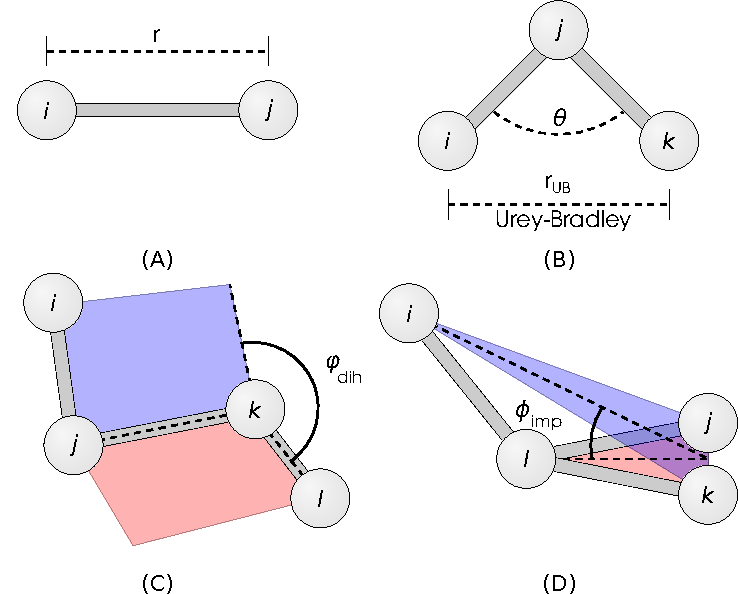
\includegraphics[width=10cm]{figures/bonded_interactions.pdf}
	\end{center}
	\captionsetup{singlelinecheck = false, justification=raggedright}
	\caption[The Bonded Interactions Calculated In Classical Forcefields]{\textbf{The Bonded Interactions Approximated In Classical Forcefields.}}{
		(A) The energy of Bond Stretching is approximated as a harmonic oscillator with respect to their separation $r$. (B) Angles between neighbouring covalently bonded atoms are also approximated as a harmonic oscillator with respect to the angle $\theta$. In some forcefields such as CHARMM there is a correction term for these angular interactions known as Urey Bradley forces. This is calculated using the separation between the non-bonded atoms $i$-$k$ in the triplet with the parameter $r_{UB}$. (C) The dihedral angle between four atoms is calculated by constructing two planes. Each plane is constructed to contains three of the four atoms in the set. One plane encompasses atoms i, j and k here  colored in blue and the other plane contains the j, k and l atoms colored in red. The dihedral angle is then calculated by taking the angle between these two planes along the line they intersect, the line formed by the j-k bond. (D) The improper dihedral angles are again calculated with the use of two planes. Containing i, j and k and j, k and l respectively. The difference is that this parameter parametrises planarity of a molecular configuration rather than the flexibility of torsion angles.
	}
	\label{charmm_bonded}
\end{figure}


In classical forcefields the non-bonded interactions are expressed using the Couloumb's law because the partial charges assigned to each atom and the Lennard-Jones potential to approximate the interactions arising from both Pauli exclusion and Van Der Walls Interactions.


\begin{equation}\label{nonbonded_eqs}
	\begin{aligned}
		U_{non-bonded} = \underbrace{\sum_{i>j} \epsilon_{ij} \Big( \Big(\frac{\sigma_{ij}}{r_{ij}}\Big)^{12} - \Big(\frac{\sigma_{ij}}{r_{ij}}\Big)^{6} \Big)}_{U_{Lennard-Jones}} - \underbrace{\sum_{i>j} \frac{q_i q_j } {r_{ij}}}_{U_{coloumb}}
	\end{aligned}
\end{equation}


The $\sigma$ parameter denotes the location of the local minima in the Lennard-Jones potential. This is the optimum distance that two atoms will rest against each other in the absence of other effects. The $\epsilon$ parameter denotes the depth of the potential well, or how stable the two atoms will be in the minimum energy configuration. This is very important for certain physical parameters such as osmotic pressure  \cite{Yoo2018}

Conversely, the partial charges in a system have the greatest influence on the solvation energy.

By focussing on these two physical parameters we can isolate and improve the non-bonded parameters.

\begin{figure}
	\begin{center}
	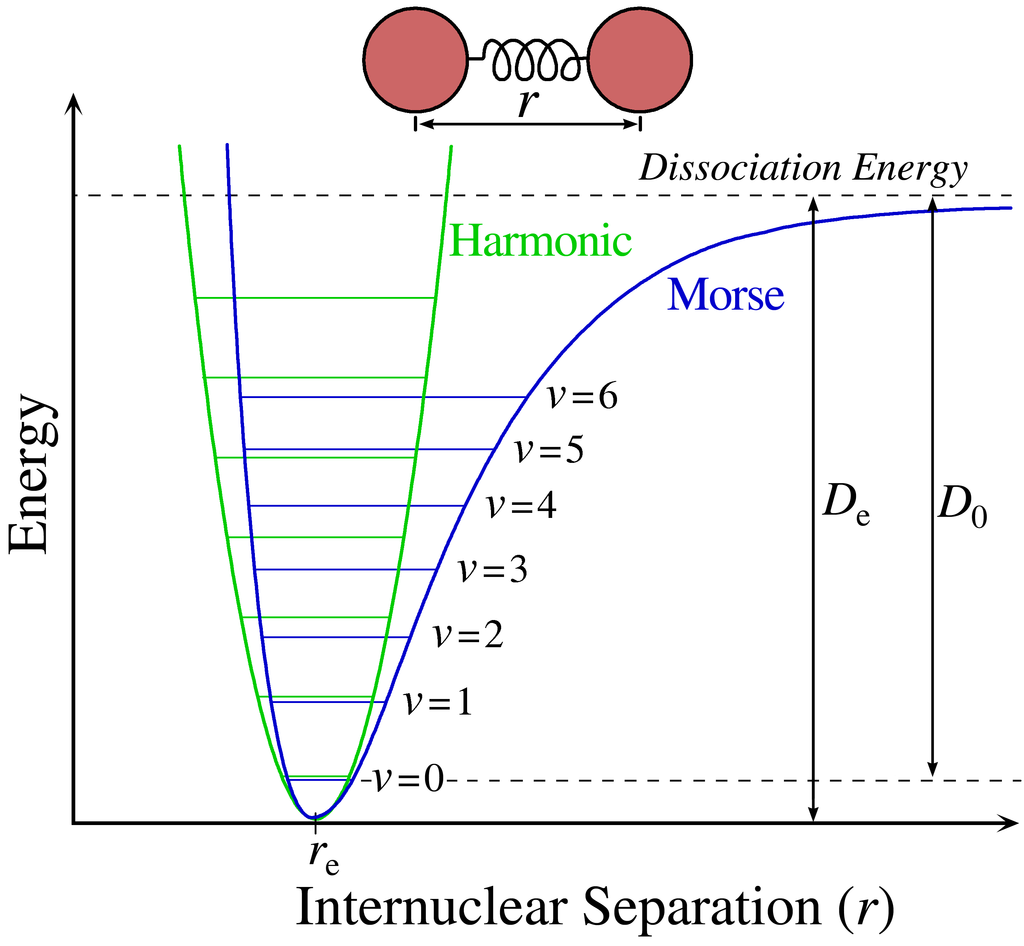
\includegraphics[width=7cm]{figures/Morse-Potential.png}
	\end{center}
	\captionsetup{singlelinecheck = false, justification=raggedright}
	\caption[The Morse Potential Compared to a Harmonic Potential] {\textbf{The Morse Potential Compared to a Harmonic Potential}}{
		The Morse potential was formulated to approximate the potential the potential energy surface of the separation of covalent bonds (blue). At low temperatures (the ground state, v=0) like those found in classical MD there is good agreement between the Morse potential and the harmonic oscillator (green). Credit Mark Somoza 2006. 
}
	\label{morse_potential}
\end{figure}

\subsection{Philosophy of Different Molecular Mechanics forcefields.}
At the time of writing, the four popular forcefields for the simulation of biomolecules are: AMBER, CHARMM, GROMOS and OPLS. Each of these have a slightly different philosophy in their formulation. They may be bottom up, as in the case of AMBER and CHARMM or top down, in the case of GROMOS and OPLS. Bottom up forcefields take the results from quantum \textit{ab initio} calculations and approximate them with the functional form mentioned above. Conversely, top down forcefields take experimental measurable such as Osmotic pressure, solvation energy. This philosophy is closest to physics 

\subsection{The Process of Preparing a Simulation}
The process of taking a molecular structure and putting it in a cellular environment to simulate it at physiological temperatures is both an art and a science. It's a science because a biophysicist must be aware of the many tricks that structural biologists use to image a macromolecular complex. But it's an art because accounting for those tricks and modifications is rarely straight forward. How do you build a missing loop? What charge state is an amino acid most likely to take during the physiological context.

\subsection{Controlling the Temperature and Pressure in a Simulation}

\subsection{Periodic Boundaries to Simulate a Realistic System Size}


\subsection{Short Comings of Classical MD}
The short comings of classical molecular dynamics fall into two classes whose solutions stand opposed to one another. These are the accuracy of the chemical forcefields outlined above and the inability of modern computers to deliver enough samples of the energy landscape to collect sufficient statistics for rigorous conclusions. The issue is that, as the above physical formulation might indicate. The more accurate the forcefields, the more computationally expensive. And so the solutions to the two are constantly in tension with one another. In the next section we will explore the current efforts to bring solutions.

\subsubsection{The Problem with Forcefields}
These approximations are not without a cost to accuracy. In certain situations, many of which are biologically relevant, it has been shown that quantum effects such as polarisation play an important role in the dynamics of the system. This has been demonstrated in the literature for Gramicidin where polarisable forcefields are able to more accurately reproduce the experimental results of current.

The other context where polarisation is important to consider are on divalent ions. Here, the solvation energy is underestimated due to the consistent lack of polarisation, making investigations of these biologically imporatnt chemical species difficult.

However, for most situations, particularly those involving bulk water and protein motions Molecular Dynamics is proving to be an invaluable tool for investigating the properties of biological systems CITATION NEEDED.  

There are several efforts to correct address these issues. These include the inclusion of the effects of polarisation, the most popular methods at the moment being adding a massless drude oscillator as an extra bead to most(?) atoms as in the CHARMM drude forcefields, championed by the Mackerell lab and the use of forcefields such as AMOEBA which explicitly calculate the dipole and quadropole moments of each atom. These both substantially increase computational cost but have displayed much better agreement with experiments in biological systems where classical forcefields have been shown to fail \cite{ngo2021}. 

Ultimately, the functional form in equation \ref{CHARMM} does not have sufficient degrees of freedom to address all possible chemical contexts  and so careful consideration must always be given to whether the forcefield is being used in a faithful way to what it was intended to simulate. So long as the user is aware of the situations where classical forcefields fall short they can be a powerful tool for the study of molecular systems.

\subsubsection{The Problem with Sampling}

To physicists the sampling is the more intuitive. Collecting sufficient statistics about the system of interest is difficult and comes at both a computational and human cost. Even though computers have sped up exponentially for the last 50 years we are still orders of magnitude from being able to reach the time scales of many biological processes. As is we struggle to sample the time scales of diffusion through an ion channel, despite the problem standing for decades. 

The slow time step demanded in classical MD due to the fast motions of certain atomic groups such as hydrogen is fundamentally at odds with the time scales of many important biological processes such as drug binding or protein folding which occur on the time scale of  milliseconds or seconds. 

Methods are now emerging which intelligently drive the simulation toward regions unexplored in the collective variable space by unbiased simulations. For some time the field has used steered methods or adaptive sampling methods such as Umbrella Sampling or Metadynamics to drive the simulation toward sections of the energy landscape which are under sampled. These methods universally rely on a choice of collective variable which closely corresponds to a slow degree of freedom. Such a choice is not usually simple. In the case of ion channels one may rationally choose the placement of the ion along the conduction pathway as the collective variable but the choice is less obvious in the case of more global conformational changes.

The advances we are seeing at the moment which I find exciting are the use of machine learning methods to tease out these degrees of freedom in order toaccelerate them with already established free energy methods. These have the potential to uncover new drug binding pockets and revolutionise our understanding of biomolecular systems. 


\subsection{Accelerating Simulations with Virtual Site Topologies}
The discrete time step, $\Delta t$ in equation \ref{verlet}, is one of the most important determinants in the performance of the simulation. We would like $\Delta t$ to be as large as possible, so that the minimum number of calculations are made to sample the desired time scale, which usually runs to nanoseconds or milliseconds.  

Due to Nyquist's theorem the $\Delta t$ parameter must be less than half the speed of the fastest degree of freedom in the system CITATION NEEDED. In the case of biomolecular systems we are challenged by the fact that they are so hydrogen-rich. Since hydrogen is so light, its motion is much faster compared to the other molecular motions involving heavier, slower moving atoms. Its correlation time is on the order of 1 femtosecond, in classical simulations we are able to get away with using 2 femtoseonds by enforcing a rigid hydrogen bond length, i.e interpolating its position backward from the 2 fs timestep.  

However, there are more involved strategies to account for these effects. Hydrogen Mass repartitioning and multiple time stepping have become popular but we will discuss Virtual Sites in detail as they were used for some simulations in this thesis.  

\begin{table}
	\begin{center}   
		\begin{tabular}{ |c|c|c|}
			Motion & Timescale
			Covalent Bond-stretching & $1-2x10^{-15}$s \\
			Covalent Bond-angular bend & $2-5x10^{-15}$s \\ 
		\end{tabular}
\end{center}
%\begin{tabular} { |c|c|c| } 
%	\hline
%	%\label{atomic_motions_speed}
%	System Description & Fastest Degree of Freedom & Characteristic Timescale \\ 
%	\hline
%	Uncoupled Atoms  & Atom Translation & 10 fs  \\ 
%	Rigid Molecules & Rigid Body Rotation & 5 fs \\  
%	Flex. Molecule with Rigid Bonds & Bond Angle Vibrations & 2 fs  \\ 
%	 Flex. Molecule with Flex. Bonds & Bond Stretching Vibrations & 1 fs  \\ 
%	\hline
%\end{tabular}
	\captionsetup{singlelinecheck = false, justification=raggedright}
	\caption[Timescales of Motions in a Molecular System]{\textbf{Timescales of Motions in a Molecular System}} {The time step of a simulation must be small enough to capture the motions in the fastest degree of freedom. In hydrogen-rich biomolecular systems the bottle neck can be found in the fast bond vibrations in lighter atoms. }
\end{table}

As you can see in table \ref{atomic_motions_speed} the fastest motion in molecular systems is dictated by the translation of hydrogen atoms. Virtual site topologies aim to remove the requirement for calculating these motions every time step by instead interpolating the positions of hydrogen atoms from the positions of surrounding heavy atoms. 

\section{Free Energy Calculations: Making Simluations More Useful}
The above work sets out how to perform unbiased MD simulations. These are powerful tools but as mentioned in section \nameref{sampling_problem} if one only relies on unbiased simulations they will quickly exceed the available computer power. So we must be clever in how we direct our available resources. This means intelligently sampling sections of the molecular phase space which are of interest to us physically but are not reached in our unbiased simulations. A technique that is used extensively throughout this thesis is the addition of a biased potential to the molecular potential $U_{MM}$ calculated for the purposes of unbiased simulations. This will drive the simulation to regions of interest. 

\begin{equation}
U_{FEC}  = U_{MM} + U_{biased} (\xi)
\end{equation}

Note how the $U_{biased}$ term is explicitly dependent on a parameter $\xi$. This parameter is known by many names, an order parameter, a collective variable or a reaction coordinate. Each of these names 

\subsection{Umbrella Sampling}

\subsubsection{Weighted Histogram Average Method}

\subsection{Metadynamics}
